\documentclass[pre,twocolumn,superscriptaddress,amsmath,amssymb,floatfix]{revtex4-2}
\usepackage{graphicx}
\usepackage{booktabs}
\usepackage[colorlinks=true,allcolors=blue]{hyperref}

\begin{document}

\title{Iterated division in living partitions: a robust degree class, and the clustering and junction geometry that tell rules apart}

\author{Alexei Vazquez}
\email{alexei@nodeslinks.com}
\affiliation{Nodes \& Links Ltd, Salisbury House, Station Road, Cambridge, CB1 2LA, UK}

\date{\today}

\begin{abstract}
Scale-rich (SR) metamaterials are planar networks built by iterated cell division: a
segment nucleates inside a cell, grows both ways to the first obstacle, and earlier
segments are thicker. In the dual graph, with segments as nodes and T-contacts as links,
the degree distribution has a $k^{-3}$ tail. We ask whether this architecture occurs in
living systems, where divisions are not sequential. With nucleation at rate $R$ per
unit area and growth at speed $v$, the control parameter is $\Pi=RL^3/v$. Parallel growth
changes only the first $n^*\simeq0.04\,\Pi^{2/3}$ segments, i.e.\ scales above
$\ell^*=(v/R)^{1/3}$; below $\ell^*$ the dual keeps $\gamma\simeq2.85$, clustering
$\langle C\rangle=0.38$ and $C(k)\sim1/k$ up to $\Pi=10^3$. The exponent $\gamma\simeq3$
is also shared by every division rule tested (cell chosen by area or uniformly, random
or centroid cuts), as the local rate-equation kernel predicts. What separates rules is
clustering and junction geometry, and turnover: uniform removal of segments cuts the tail
at $k\approx25$--$35$, while removal suppressed for highly connected segments restores it.
We test three biological partitions. Plant cell walls in six shoot apical meristems
(4~h time-lapse with lineage) form an iterated division with no corner cuts (0 of 672
divisions; SR gives 0.21), the side distribution of Errera's shortest-wall rule
(total-variation distance 0.03), and junctions born at $\theta\simeq143^\circ$ that relax
toward $120^\circ$; a vertex model in which a new wall starts at $t_0\simeq0.6$--$0.75$
of the mature tension and matures over $\tau\simeq24$--$48$~h, about one cell cycle
$T_{cc}\simeq36$~h, reproduces the angle-age curve within $2^\circ$ and predicts dual
clustering $0.20$--$0.23$, against $10^{-3}$ without relaxation. In six flower-meristem
films, with no parameter adjusted, the fraction of new walls that land on two already
linked walls is $0.19\pm0.06$, against $0.19$ predicted with relaxation and $0.002$
without: junction relaxation creates the dual clustering of plant walls. Leaf minor venation
carries the SR thickness hierarchy (the collinear pair at a junction is thicker than
the stem in $78\%$ of cases) and a nested loop hierarchy without the small-split excess
of random partitions, but its dual degree law cannot be separated from the vein
construction. The ventral actin network of COS-7 cells is a crossing mesh rather than a
T-partition at the resolution analysed.
\end{abstract}

\maketitle

\section{Introduction}

Scale-rich (SR) metamaterials~\cite{both2026} are ligament networks grown by a simple
rule: a point is drawn at random, a segment at a random angle grows from it in both
directions until it meets the existing structure, and segments are thinner the later
they are born. Geometrically the construction is Cowan's iterated cell
division~\cite{cowan2010}, a relative of the STIT tessellation~\cite{nagel2005}. As a
graph, the dual (segments as nodes, T-junctions as links) has a degree distribution
$p_k=12/[k(k+1)(k+2)]$, which follows from a rate equation with an attachment kernel
$(a+bk)/t$ deduced from local face sampling, $b=2/\langle n\rangle=1/2$ and
$a=0$~\cite{krapivsky2000,vazquezbook,vazquez2026sr}. The clustering spectrum
$C(k)\simeq2p/k$ is set by the probability $p$ that a new segment cuts a corner of its
cell~\cite{vazquez2026sr}.

Living matter is full of planar partitions built by insertion: new plant cell walls
expand outward from the division site until they fuse with the parental
walls~\cite{besson2011}, leaf veins form a hierarchy in which thinner veins end on
thicker ones~\cite{couder2002,bohn2002}, and actin bundles in spread cells are nucleated,
elongate and terminate on other bundles~\cite{tojkander2015,vignaud2021}. None of these
processes is sequential. Many compartments divide at the same time, segments grow at a
finite speed, division planes follow rules other than a random angle, and the material
turns over. The questions are therefore (i) which features of the SR class survive these
relaxations, (ii) which observables distinguish the rules, and (iii) what real
partitions show.

Section~\ref{sec:model} introduces parallel nucleation and shows that it changes only
the top of the hierarchy. Section~\ref{sec:rules} shows that $\gamma\simeq3$ is shared by
all division rules tested and that turnover is the main threat to the tail.
Section~\ref{sec:images} describes the image and graph analysis.
Sections~\ref{sec:actin}--\ref{sec:refahi} report actin in flat cells, leaf venation,
shoot apical meristems, a plant-specific vertex model, and a parameter-free test of that
model on flower meristems.

\section{Iterated division with parallel nucleation}
\label{sec:model}

\paragraph*{Model.} In a square of side $L=1$, segments nucleate as a Poisson process of
rate $R$ per unit area per unit time, at a uniform point and a uniform angle. Each
segment grows in both directions at speed $v$. A tip stops where it first meets a
segment that is already there, finished or still growing, or the boundary; when two
growing segments cross, the later arrival stops. The simulation is exact and event
driven. All junctions are T-junctions, and every stopped tip lies on its target. The
dimensionless control parameter is
\begin{equation}
\Pi=\frac{RL^3}{v},
\end{equation}
the number of nucleations while a tip crosses the domain. $\Pi\to0$ is the sequential SR
process; $\Pi\gg N^{3/2}$, with $N$ the final number of segments, is the Gilbert
tessellation~\cite{gilbert1967}, in which all segments nucleate before any stops.

\paragraph*{Local criterion.} When $n$ segments are present, a typical cell has size
$\ell=n^{-1/2}$ and is crossed in time $\ell/v$. The number of nucleations inside it
during that time is $R\ell^2\cdot\ell/v=\Pi\,n^{-3/2}$. Growth is effectively sequential
once this number is below one, i.e.\ for
\begin{equation}
n>n^*\sim\Pi^{2/3},\qquad \ell<\ell^*=(v/R)^{1/3}.
\end{equation}
Parallel growth therefore affects only the first $n^*$ segments, the top of the
hierarchy, and leaves the SR statistics at all smaller scales.

\paragraph*{Simulations.} With $N=2\times10^4$ segments and three realizations
(Fig.~\ref{fig:model}a), $\Pi=10^{-3}$ to $10^3$ gives $\gamma=2.82$--$2.87$ (maximum
likelihood, $k\geq10$), $\langle C\rangle=0.376$, $C(k)\sim1/k$, a triangle-closure
probability of $0.49$ per new segment, and a correlation $0.94$ between $k-2$ and
length $\times$ age, all as in sequential SR. At $\Pi=10^4$ the largest degree is
$k_{\max}=65$ against $281$ for $\Pi=10^{-3}$, and at $\Pi=10^6$ (where $n^*\sim N$) the
network is Gilbert-like, with $\gamma>4$ ($9.05$ for $k\geq10$, $4.61$ for $k\geq6$),
$k_{\max}=16$ and $\langle C\rangle=0.26$. The crossover rank, defined as the birth rank
at which the cohort mean degree reaches half its $\Pi\to0$ value
(Fig.~\ref{fig:model}b), is $n^*/\Pi^{2/3}=0.024$, $0.038$ and $0.055$ for $\Pi=10^3$,
$10^4$ and $10^6$, consistent with $n^*\simeq0.04\,\Pi^{2/3}$.

\begin{figure*}[t]
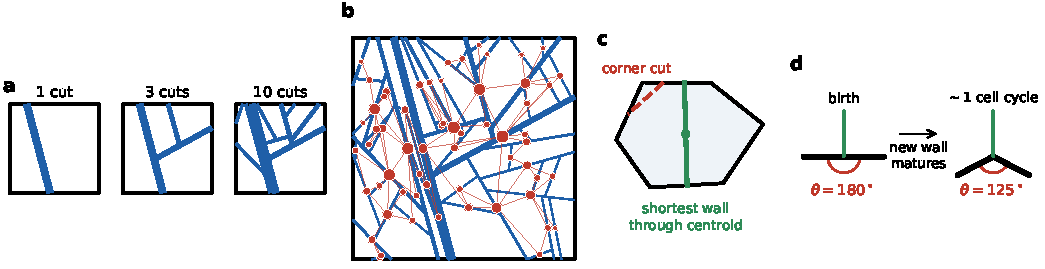
\includegraphics[width=\textwidth]{figs/fig1.pdf}
\caption{Iterated division with parallel nucleation and turnover. (a) Degree exponent
$\gamma$ ($k\geq10$, circles, left axis) and mean clustering $\langle C\rangle$ (squares,
right axis) of the dual against $\Pi=RL^3/v$; $N=2\times10^4$, three realizations.
(b) Mean degree of segments of birth rank $i$ relative to $\Pi\to0$. Inset: crossover
rank $n^*$ (ratio $=1/2$) against $\Pi$; line $0.04\,\Pi^{2/3}$. (c) Degree
distribution in the steady state with turnover ($n_{ss}=1500$, $\Pi=0.01$): uniform
removal ($s=0$) and removal rate $\propto(2/k)^s$ ($s=1,2$; $n\approx1500$), against SR without
turnover at $N=1500$.}
\label{fig:model}
\end{figure*}

\section{Division rules and turnover}
\label{sec:rules}

\paragraph*{Rules.} Iterated division has three choices: which cell divides, where the
cut passes, and at which angle~\cite{cowan2010}. We compared, at $N=2\times10^4$, SR (cell
$\propto$ area, uniform point, uniform angle), equal per-cell clocks (cell chosen
uniformly), centroid cuts at a uniform angle, and a balanced rule (centroid,
perpendicular to the major axis, Errera-like~\cite{errera1888,besson2011}). All give
$\gamma=2.89$--$3.06$ ($k\geq10$). This is consistent with the rate-equation argument: a segment
of degree $k$ borders about $k$ cells and is reached through them, so the attachment rate is
linear in $k$ for any of these rules, with a slope set by the mean number of sides rather
than by how the cell or the cut is chosen. The rules differ in clustering, $\langle C\rangle=0.38$, $0.45$,
$0.28$ and $0.055$ respectively, and in the spread of segment lengths, $\mathrm{sd}(\ln
L)=0.86$, $3.3$, $0.69$ and $0.59$. Clustering is set by the corner-cut probability: a
balanced cut through the centroid rarely joins two adjacent sides.

\paragraph*{Turnover.} Actin bundles turn over on a minute
scale~\cite{tojkander2015}. We removed each segment at rate $\delta$; tips that had
stopped on a removed segment resume growth. The steady state holds $n_{ss}=R/\delta$
segments. With uniform removal at $n_{ss}=1500$, $P(k\geq16)=0.003$--$0.008$ and
$k_{\max}=22$--$26$ for $\Pi=0.01$, $100$ and $3000$, against $P(k\geq16)=0.021$ and
$k_{\max}=82$ for SR with $N=1500$ and no turnover (Fig.~\ref{fig:model}c). The cutoff
barely depends on $n_{ss}$ ($k_{\max}=18$, $22$, $27$ at $n_{ss}=300$, $1500$, $4000$)
because a segment's mean lifetime always spans $n_{ss}$ nucleations: uniform turnover
produces a characteristic degree. If removal is suppressed for highly connected segments,
with rate $\delta(2/\max(k,2))^s$ and $\delta$ rescaled to keep $n\approx1500$, the tail
returns: for $s=1$, $2$, $3$ ($n=1438$, $1456$, $1583$) $P(k\geq16)=0.016$, $0.016$, $0.020$
and $k_{\max}=60$, $75$, $67$. The correlation between degree and age is $0.61$--$0.71$ in all
turnover runs. A scale-rich cytoskeleton would thus require load-dependent stability of
bundles.

\section{From images and graphs to the dual}
\label{sec:images}

\paragraph*{Pipeline.} For fluorescence images: a ridge filter, a threshold and a
skeleton; junction clusters joined by branches shorter than 8~px are merged; the
direction of each arm is fitted on skeleton pixels 6--18~px from the junction. A
3-arm junction is a T if two arms are collinear within $25^\circ$ and a Y otherwise; a
4-arm junction with two collinear pairs is an X. Branches are merged through collinear
pairs into lines, and the dual links the stem line to the through line at each T. For
segmented tissues (label images) the same classification runs on walls between cells,
and for vein graphs on the edges with their recorded end orientations.

\paragraph*{Validation.} On rendered model networks ($1024^2$~px, blur $1.5$~px, noise),
the T share among 3-arm junctions is $0.87$--$0.97$ for SR and Gilbert networks, and the
number of X per junction is $0.04$--$0.06$, against $0.16$--$0.32$ for random rods that
cross freely. The degree tail is undercounted: $P(k\geq4)=0.15$--$0.17$ against true
values $0.27$--$0.31$, and $k_{\max}$ is about one third of the true one, so exponents
from images are biased upward. On rasterized model tissues the label-image route
recovers the dual: for SR, $P(k\geq4,8,16)=0.30,0.085,0.023$ against true
$0.29,0.085,0.026$, $\langle C\rangle=0.36$ against $0.38$, and $3.97$ geometric corners
per cell against $4$.

\section{Actin in flat cells}
\label{sec:actin}

No public set of whole spread human cells resolves stress fibres at a resolution
suitable for junction statistics; the closest is BioSR~\cite{qiao2021}: 51 COS-7 cells
with Lifeact, TIRF-SIM, $31.3$~nm per pixel, ventral plane. Over all cells the pipeline
finds 11389 junctions: 4192 T, 2652 Y, 772 X and about 1900 clusters with $\geq5$ arms.
$T/(T+Y)=0.61$ and X per junction $0.068$. The skeleton is fragmented (62791 line pieces,
$P(k\geq2)=0.07$), and the partial correlation between degree and bundle width at fixed
length is $0.05$. The image (Fig.~\ref{fig:actin}) shows long curved bundles that cross
at shallow angles over a dense meshwork: a crossing mesh, not a T-partition. The
segmentation is untuned and the cells are not human, so this result is a first pass. It
is consistent with the literature: Arp2/3 branches are one-sided Y-junctions at about
$70^\circ$, dorsal fibres grow one way from adhesions, and arcs thicken by lateral
fusion~\cite{tojkander2015}; ventral fibres are embedded in a contractile cortical
mesh~\cite{vignaud2021}. Keratin networks have a mean vertex degree of
$3.5$--$4.2$~\cite{luck2010}, above the value $3$ of a T-partition. Two cautions apply to
future analyses: tracing algorithms that stop a curve when it meets another, such as
SOAX~\cite{xu2015soax}, create T-junctions by construction; and cortical actin
compartments, whose areas are log-normal and have been read as successive fragmentation
by growing filaments~\cite{sadegh2017}, are the closest published analogue and have not
been compared with iterated-division statistics.

\begin{figure}[t]
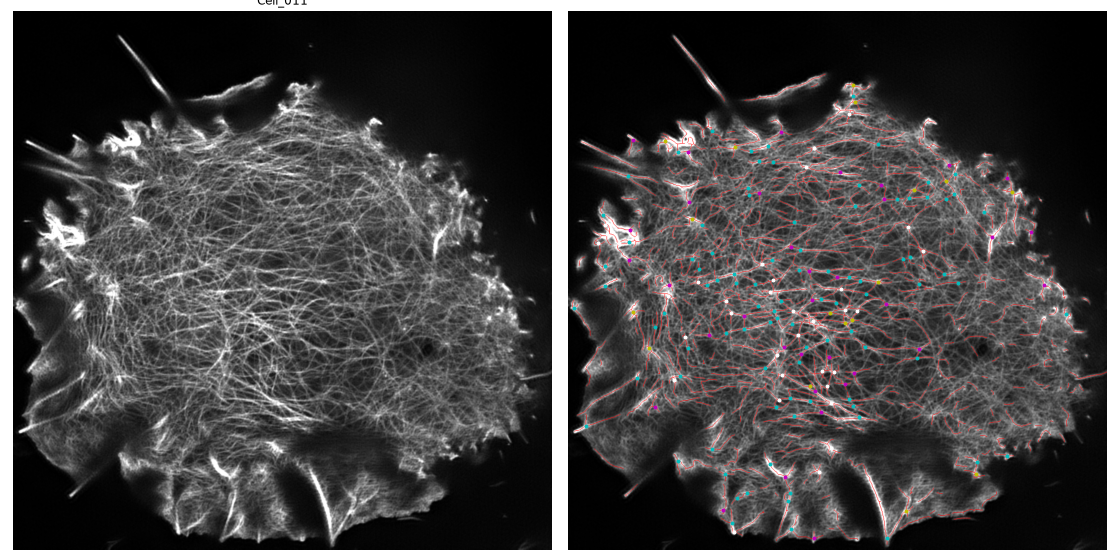
\includegraphics[width=\columnwidth]{figs/fig4.png}
\caption{F-actin in a COS-7 cell (BioSR Cell\_011, Lifeact, TIRF-SIM, field $31$~$\mu$m).
Left: image. Right: skeleton (red) with T (cyan), Y (magenta) and X (yellow) junctions.
Bundles cross at shallow angles over a dense meshwork.}
\label{fig:actin}
\end{figure}

\section{Leaf venation}
\label{sec:venation}

\paragraph*{Data.} LeafVeinCNN~\cite{xu2021} provides extracted vein graphs with
per-edge widths for cleared-leaf segments of about $1$~cm$^2$; we used the 44 segments
of one plot (25 species, 283380 vein edges). The graphs include the hierarchical loop
decomposition (HLD), the binary tree obtained by fusing adjacent loops in order of
increasing width of the vein between them.

\paragraph*{Junctions.} Of the vein nodes, $34\%$ are free ends (free-ending veinlets,
absent in SR). At 3-way nodes the largest angle between arms has median $147^\circ$, and
$32\%$ exceed $155^\circ$ (Fig.~\ref{fig:venation}a): junction geometry lies between T and
Y, as expected when junction angles follow vein radii~\cite{bohn2002}. The width
hierarchy agrees with the geometry: at geometric T's the stem is the thinnest arm in
$78\%$ of cases, and at all 3-way nodes of the loop network the arm opposite the widest
gap is the thinnest in $71\%$ (67926 nodes), against $1/3$ for widths unrelated to
geometry. This is the SR property that a segment ends on an older, thicker one.

\paragraph*{Loop nesting.} For SR with widths ordered by birth, the HLD is the division
tree read backwards, and the smaller-child area fraction is uniform on $[0,1/2]$ (mean
$0.25$; Fig.~\ref{fig:venation}b). Centroid and balanced cuts put almost all splits
above $0.45$ (means $0.47$, $0.48$). The leaves give mean $0.28$ and quartiles
$0.16$/$0.30$/$0.41$ over 20112 fusions, a smooth rise toward $1/2$ and no excess of
very small splits. A Voronoi tiling fused with random widths, and SR with noisy widths
(lognormal noise of unit standard deviation on the birth-ordered widths), both show such
an excess, with lower quartiles $0.047$ and $0.076$. The loop nesting is therefore that
of an ordered sequential subdivision, with a mild bias toward even splits.

\paragraph*{Dual degree law: not identifiable.} Because junction angles do not define
lines, we built lines by width continuation (the two widest arms continue through a node,
the others are stems). On the loop network this gives $P(k\geq4,8,16)=0.31,0.066,0.008$,
$C(k)=0.43$, $0.24$, $0.15$, $0.09$, $0.05$, $0.03$ for $k$ in the bins starting at $2$,
$3$, $5$, $8$, $13$, $21$, and a partial correlation $0.40$ between $\ln k$ and $\ln W$ at
fixed $\ln L$. The same construction on a Voronoi tiling with random widths gives
$P(k\geq4)=0.30$, $C(k)$ from $0.34$ to $0.04$ and a partial correlation $0.32$; on SR
with birth-ordered widths the partial correlation is $0.57$. The degree law and $C(k)$ of
the venation dual are therefore produced by the line construction itself and are not
evidence for the SR class; only the width--degree correlation lies slightly above the
null. The longest, oldest veins cross the sample boundary and are excluded, which also
truncates the tail.

\begin{figure*}[t]
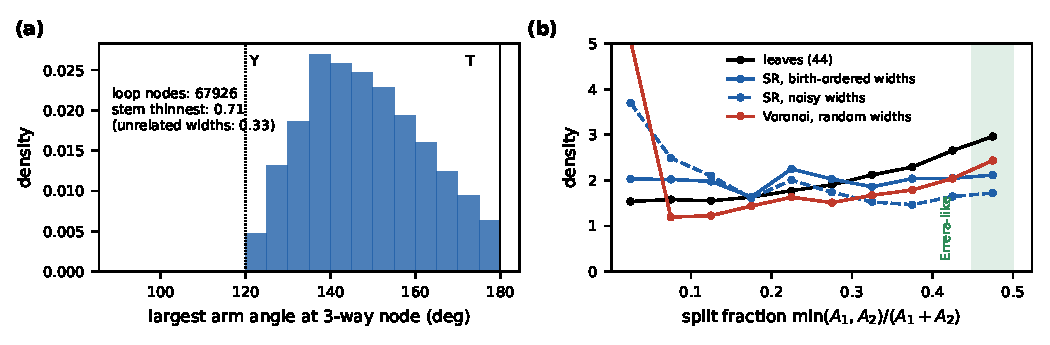
\includegraphics[width=\textwidth]{figs/fig2.pdf}
\caption{Leaf venation (44 LeafVeinCNN segments). (a) Largest arm angle at interior
3-way nodes of the loop network; $180^\circ$ is a T, $120^\circ$ a symmetric Y. (b)
Smaller-child area fraction at the fusions of the hierarchical loop decomposition: leaves
against SR with birth-ordered widths, SR with noisy widths and a Voronoi tiling with
random widths (rasterized, $T=800$ cells, three realizations). The shaded band marks where
centroid and balanced division rules put almost all splits.}
\label{fig:venation}
\end{figure*}

\section{Shoot apical meristem walls}
\label{sec:sam}

\paragraph*{Data and wall identity.} Willis \textit{et al.}~\cite{willis2016} imaged six
\textit{Arabidopsis} shoot apical meristems every 4~h for 76--84~h and tracked the L1
cells. We projected the L1 layer to a label image at each time point and extracted walls
and triple junctions. Wall identity follows from the lineage: the wall between cells $a$
and $b$ at $t+4$~h belongs to the line of the wall between their mothers at $t$, unless
both have the same mother, in which case it is a new division wall. For each division the
host lines are the lines of the mother's walls on which the new wall ends. Of 1117
divisions in low-slope regions, 672 have both hosts identified.

\paragraph*{No corner cuts.} A new wall cuts a corner if its two hosts are adjacent sides
of the mother, i.e.\ meet at one of its vertices. This happens in $0$ of $672$ divisions
($95\%$ upper bound $0.45\%$). On the same topological definition SR gives $0.21$ and
Errera's shortest wall through the centroid gives $0$ (Sec.~\ref{sec:plantmodel}). The
detector is calibrated: $44\%$ of the neighbour pairs of a cell meet at one of its
vertices, close to $2/(n-1)$.

\paragraph*{Junction angles.} The angle $\theta$ between the two host pieces at a new
junction is $180^\circ$ for a straight T. At the first observation (age $0$--$4$~h)
$\theta$ has median $143^\circ$ (quartiles $135^\circ$/$143^\circ$/$151^\circ$; $3.6\%$
above $165^\circ$), and it decreases with age to $128^\circ$ at $36$--$40$~h, in all six
plants (Fig.~\ref{fig:sam}a). Straight wall lines therefore dissolve into Y-junctions
within about one cell cycle.

\paragraph*{Topology.} Without neighbour exchange, a division of a cell with $n$ sides
into daughters with $n_1$ and $n_2$ sides satisfies $n_1+n_2=n+4$, and if no division cuts
a corner no cell ever has three sides. Over 12182 observations of interior low-slope
cells, $P(n)$ for $n=3$--$9$ is $0.003$, $0.041$, $0.267$, $0.408$, $0.230$, $0.046$,
$0.003$; $n_1+n_2-n$ has mode $4$ in every plant (values $5$, $6$ arise when a neighbour
divides in the same interval). Between $6.4\%$ and $12.2\%$ of tracked cells divide per
4~h interval, which for asynchronous exponential growth gives a cell cycle
$T_{cc}=4\ln2/\ln(1+f)=24$--$45$~h (median $36$~h).

\paragraph*{Degree law: not testable.} In 76~h cells divide at most about twice, wall
identity breaks where lineage is missing, and the largest observed line degree is $6$.

\section{A plant division model}
\label{sec:plantmodel}

\paragraph*{Model.} Cells are polygons with shared vertices in a square. A cell is chosen
with probability $\propto A^4$ (size-threshold-like) or $\propto A$. The new wall passes
through the centroid along the shortest of 36 directions whose ends lie at least $0.15$
wall lengths from existing vertices (no four-way junctions); a no-corner-cut constraint
is available but never binds (below). Mechanics is a quasi-static vertex model,
\begin{equation}
E=\sum_e T_e\,\ell_e+\sum_c\frac{K}{2}\frac{(A_c-A_c^0)^2}{(A_c^0)^{3/2}},
\end{equation}
with $A_c^0$ the area at birth, $K=20$, mature tension $1$, and a new wall whose tension
matures with age $a$ as
\begin{equation}
T(a)=1-(1-t_0)\,e^{-a/\tau}.
\end{equation}
At a fresh junction force balance gives $\theta=2\arccos(t_0/2)$; $t_0=0.6$ gives
$145^\circ$ in the simulation. Time advances by $1/N$ per division, so one unit is
$T_{cc}/\ln2$ with $T_{cc}=36$~h. Each wall carries the identity of the division that
created it, so the dual is defined exactly.

\paragraph*{Corner cuts and $P(3)=0$.} Errera's shortest wall never cuts a corner,
with or without the explicit constraint; $P(3)=0$ and $n_1+n_2=n+4$ hold exactly. With
random cuts (SR rule) the corner-cut probability is $0.21$ and $P(3)=0.09$.

\paragraph*{Junction angles.} Fitting $(t_0,\tau)$ to the meristem angle--age curve
over a $4\times4$ grid (two realizations of 600 cells each) gives a shallow valley:
$(t_0,\tau)=(0.6,24~\mathrm{h})$ with rms deviation $1.9^\circ$ and $(0.75,48~\mathrm{h})$
with $1.7^\circ$, while fast maturation, $(0.3,8~\mathrm{h})$, gives $6.2^\circ$
(Fig.~\ref{fig:sam}a). A new wall starts at about two thirds of the mature tension and
matures over about one cell cycle.

\paragraph*{Side distribution.} At $N=2000$ (two realizations, Fig.~\ref{fig:sam}b),
Errera division without relaxation gives $P(n)$ at total-variation distance $0.03$ from the
meristem data, Errera division with the fitted tension maturation $0.11$ (too many
hexagons), with area-proportional choice $0.16$, and SR $0.37$. Raising the area stiffness
to $K=100$ lowers the distance to $0.05$ but raises the angle rms to $3.9^\circ$. The
division geometry alone therefore accounts for the meristem $P(n)$, while an
equal-tension vertex model that reproduces the junction angles over-regularizes the
cells. The influence of division rules on $P(n)$ has been studied
before~\cite{gibson2006,sahlin2010}; the new elements here are the wall-line dual and the
tension maturation.

\paragraph*{Dual predictions.} All variants give $\gamma=2.84$--$3.01$ ($k\geq6$): plant
walls are in the degree class of SR. Clustering separates the mechanics:
$\langle C\rangle=0.0008$ for Errera division without relaxation, $0.20$--$0.23$ with
relaxation, with $C(k)\sim1/k$, and $0.36$ for SR. In the relaxed model a new wall lands on
two host lines that are already linked in $27$--$31\%$ of divisions ($K=100$ and $20$),
against about $0$ without relaxation: relaxation bends lines so that the two sides
selected by the shortest wall can belong to lines that meet elsewhere. In the 76~h shoot-meristem
films only four divisions have both hosts dated (one linked); the longer flower-meristem
films test the prediction (Sec.~\ref{sec:refahi}).

\begin{figure*}[t]
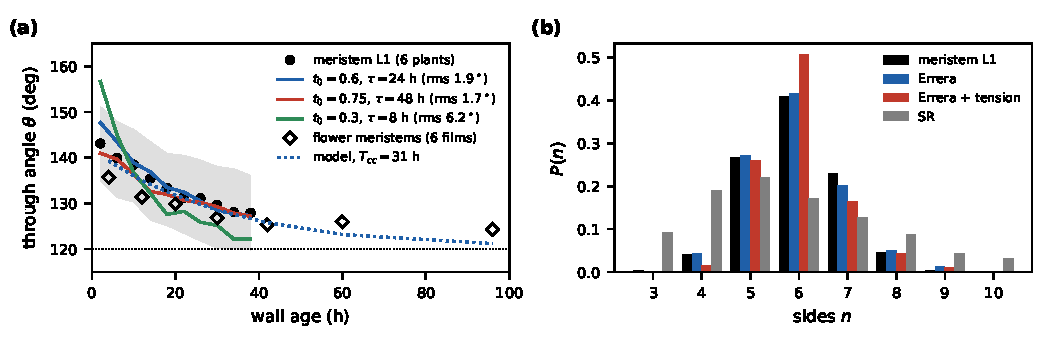
\includegraphics[width=\textwidth]{figs/fig3.pdf}
\caption{Shoot apical meristem L1 against the plant division model. (a) Through angle
$\theta$ at the junctions of new walls against wall age: shoot meristems, medians (dots)
and quartiles (band) over six plants; flower meristems, medians over six films
(diamonds); lines, vertex model with tension maturation $(t_0,\tau)$ fitted on the shoot
meristems ($T_{cc}=36$~h), and the same model at $t_0=0.7$, $\tau=36$~h with
$T_{cc}=31$~h (dotted).
(b) Side distribution $P(n)$: meristem (12182 cell observations), Errera division
without relaxation, Errera division with fitted tension maturation ($t_0=0.7$,
$\tau=36$~h), and SR ($N=2000$, two realizations).}
\label{fig:sam}
\end{figure*}

\section{Flower meristems: a parameter-free test}
\label{sec:refahi}

Refahi \textit{et al.}~\cite{refahi2021} tracked all cells of wild-type flower meristems
with 4--13~h steps. We analysed the L1 layer of six films (FM1 0--132~h, FM5 16--173~h,
the others 55--69~h), with wall identity propagated through the lineage as in
Sec.~\ref{sec:sam}; 3008 new L1 walls have identified host relations. Intervals longer
than a cell cycle (three to six daughters per mother) leave the internal order of
divisions undetermined, so the corner-cut test uses only two-daughter divisions. The cell
cycle, from the summed intervals over the summed $\log_2$ of daughter numbers, is
$T_{cc}=31.4$~h.

\paragraph*{Corner cuts.} $4$ of $252$ decidable divisions cut a corner ($1.6\%$), against
$0/672$ in shoot meristems and $0.21$ for SR.

\paragraph*{Dual clustering.} The host-linked fraction is the probability that a new wall
lands on two host lines already linked in the dual. It is decidable when both hosts were
born in the film before the new wall and their own hosts are known. Under this
restriction the data give $0.19\pm0.06$ ($n=47$). The plant model with the tension fitted
on the shoot-meristem angles ($t_0=0.7$, $\tau=36$~h), $T_{cc}=31$~h and the same
restriction over a 150~h window gives $0.19$ with relaxation ($K=20$ and $100$) and $0.002$
without. No parameter is adjusted to the flower data: junction relaxation is what creates
dual clustering in plant walls, and its measured amount is the one the angle relaxation
implies.

\paragraph*{Junction angles.} The through angle $\theta$ has median $135.7^\circ$,
$131.4^\circ$, $129.9^\circ$, $126.9^\circ$, $125.3^\circ$, $126.0^\circ$ and $124.3^\circ$
for ages in $[0,8)$, $[8,16)$, $[16,24)$, $[24,36)$, $[36,48)$, $[48,72)$ and $[72,120)$~h
(Fig.~\ref{fig:sam}a). The model ($K=20$) gives $139.3^\circ$, $135.0^\circ$,
$131.8^\circ$, $128.5^\circ$, $125.8^\circ$, $123.2^\circ$ and $121.2^\circ$: agreement
within $4^\circ$ up to $48$~h, after which the data level off near $125^\circ$ while the
model approaches the equal-tension value $120^\circ$.

\paragraph*{Degree against age.} For film-born lines with known hosts, the mean degree is
$2.38$, $3.07$, $3.84$, $3.14$ and $2.84$ for line ages $0$--$20$, $20$--$40$, $40$--$70$,
$70$--$110$ and $110$--$200$~h; the model gives $2.04$, $2.69$, $3.50$, $5.0$ and $8.2$
(last bin $110$--$150$~h). The two agree up to $70$~h; older data lines are censored,
because walls that later abut them belong to cells outside the tracked L1 region. The
largest observed degree is $12$, so the degree law remains untestable on these films.

\section{Discussion}

The SR class of iterated division is robust in the two respects that matter for living
matter. Parallel nucleation at finite growth speed leaves every scale below
$\ell^*=(v/R)^{1/3}$ unchanged and alters only the first $n^*\simeq0.04\,\Pi^{2/3}$
segments; and the degree law $\gamma\simeq3$ is shared by every division rule tested,
because the attachment kernel is set by local face sampling and the mean number of sides.
The degree law therefore cannot identify a rule. Clustering and junction geometry can:
the corner-cut probability sets $C(k)$, and the junction angle records whether segment
identity survives. Turnover is the one ingredient that removes the tail, unless highly
connected segments are protected.

Plant cell walls are the clearest living iterated division. Lineage gives every wall a
birth time, and the meristem data fix the rule (no corner cuts, as Errera's shortest
wall implies) and the mechanics (new walls at $t_0\simeq0.6$--$0.75$ of mature tension,
maturing over $\tau\simeq T_{cc}$). The model places plant walls in the $\gamma\simeq3$
class with dual clustering that measures junction relaxation, and the flower meristems
confirm the prediction without free parameters (host-linked fraction $0.19\pm0.06$
against $0.19$, and $0.002$ without relaxation); the degree law itself awaits films that
follow walls over several cell cycles; the side distribution
follows from the division geometry, while the equal-tension relaxation that fits the
angles over-regularizes cells, so an ingredient that bends junctions without
regularizing cells (for example wall-specific tensions or anisotropic growth) is
missing. Leaf veins carry the SR hierarchy, thinner veins ending on thicker ones and
loops nested as an ordered subdivision, but their dual degree law is not identifiable
from $1$~cm$^2$ samples, since width-continued lines produce the same statistics on a
random tiling. Whole-leaf graphs, in which the oldest veins are not cut by the sample
boundary, are the natural next test. The ventral actin network of COS-7 cells is a
crossing mesh at the resolution analysed; the model locates what a scale-rich
cytoskeleton would require, namely $\Pi$ small enough below the cell size and
load-dependent bundle stability, and the observables to test it: the X fraction, the
T share, stem-versus-through widths and, with time-lapse data, the degree against bundle
age.

\section*{Data and code availability}

Code and results are in the \texttt{bio/} folder of the repository: parallel-division
simulation \texttt{model/pargrow.py} (scan \texttt{model/scan.py},
\texttt{results/scan\_N20000.json}; crossover \texttt{model/crossover.py}); division
rules \texttt{model/percell.py}; turnover \texttt{model/turnover.py}
(\texttt{results/turnover\_nss1500*.json}); image pipeline \texttt{images/pipeline.py},
validation \texttt{images/validate.py} and \texttt{images/validate\_tissue.py}; BioSR
analysis \texttt{images/run\_biosr.py} (\texttt{results/biosr\_summary.json}); venation
\texttt{images/venation.py}, \texttt{images/venation\_angles.py},
\texttt{images/venation\_width.py}, nulls \texttt{images/hld\_null.py} and
\texttt{images/width\_lines\_null.py}; meristem \texttt{images/meristem.py} and
\texttt{images/meristem\_topo.py} (\texttt{results/meristem\_*.json}); flower meristems
\texttt{images/refahi.py}, \texttt{images/refahi\_stats.py}
(\texttt{results/refahi\_stats.json}, \texttt{results/refahi\_FM*.json}) and
\texttt{model/refahi\_model.py} (\texttt{results/refahi\_model.json}); plant model
\texttt{model/plantdiv.py}, fit \texttt{model/fit\_tension.py}
(\texttt{results/fit\_tension.json}), predictions \texttt{model/predict\_plant.py}
(\texttt{results/plant\_predictions\_N2000.json}) and \texttt{model/stiff.py}; figures
\texttt{figures.py}. Printed outputs of the scripts are stored as \texttt{results/*.txt}. Data: BioSR (doi:10.6084/m9.figshare.13264793), LeafVeinCNN
(doi:10.5281/zenodo.4008361), Willis \textit{et al.}\ (doi:10.17863/CAM.7793), Refahi
\textit{et al.}\ (doi:10.17863/CAM.61991).

\bibliography{references}

\end{document}
